\documentclass[FinalReport.tex]{subfiles}
\begin{document}
For controllers that takes into account few past observations only, solutions are heavy tailed. Taking the extreme case $n=1$ we propose a natural modification to hinder extreme deviations. When $\abs{z_t/z_{t-1}}$ exceeds a threshold $\varepsilon>0$ it is replaced by a positive constant $\eta$. This constant step must be taken in the right direction (i.e. such that $c_t$ gets closer to $\alpha_0$), which is given by the sign of $z_t/z_{t-1}$ (see Figure \ref{fig:new_cont_scheme}). The new map reads:
\begin{subequations}
\begin{align}	
	z_{t+1}&=(\alpha_0-c_t)z_t+\beta_t\\
	c_t&=
\begin{cases}\label{eq:nc_eta}
	c_{t-1}+\frac{z_t}{z_{t-1}},\quad &\abs{\frac{z_t}{z_{t-1}} }<\varepsilon\vspace{.1cm} \\ 
	c_{t-1}+\eta\,\sign{\frac{z_t}{z_{t-1}}},\quad &\abs{\frac{z_t}{z_{t-1}} }>\varepsilon .
\end{cases}
\end{align}
\label{eq:nc}
\end{subequations}
\eqref{eq:nc_eta} is similar to a line search strategy, where $\sign{z_t/z_{t-1}}$ is the descent direction and $\eta$ a constant learning rate.

\begin{figure}
\centering
\makebox[\textwidth][c]{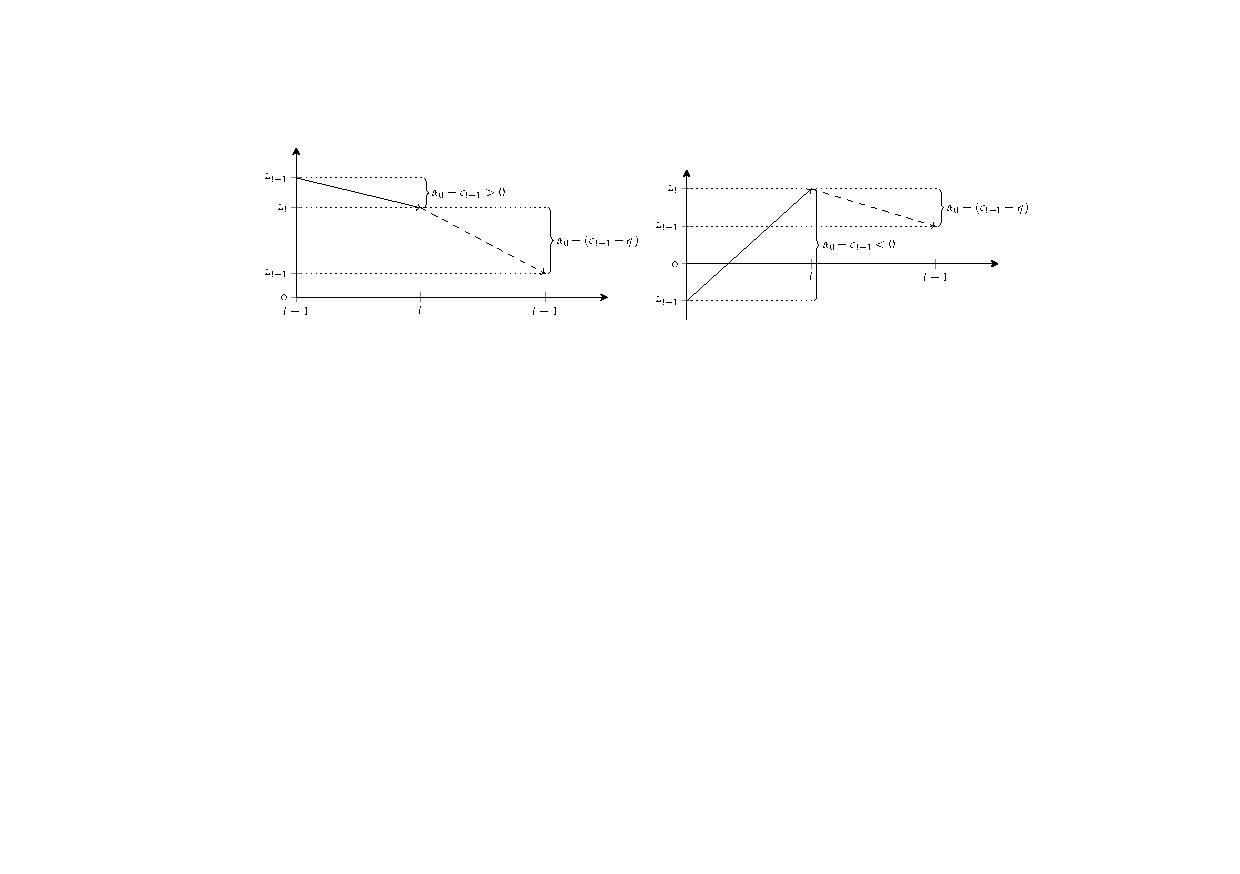
\includegraphics[width=1.2\textwidth]{Graphs/control.pdf}	}
\caption{Schematic representation of the modification proposed. Left: $\sign{\frac{z_t}{z_{t-1}}}=1$, Right: $\sign{\frac{z_t}{z_{t-1}}}=-1$. At each time step a constant is either added or subtracted to the previous estimate, in order to minimize the error $\abs{\alpha_0-c_t}$.}
\label{fig:new_cont_scheme}
\end{figure}
Final distribution depends heavily on the choice of those two parameters. From simple heuristic arguments one can reduce the range of parameters to consider: First, when $\varepsilon$ is too large, regularization is rarely engaged hence results are unchanged. We therefore restrict the analysis to $\varepsilon<1$, meaning that original controller is always replaced when the time series is growing ($\abs{z_t/z_{t-1}}>1$). Secondly, $\eta$ gives the maximal precision the estimator can achieve on $\alpha_0$, and should thus be small enough. As for $\varepsilon$, we only consider $\eta<1$.



\section{Numerical results}
Figure \ref{fig:quant_max} shows the maximum value and $99\%-$quantile of time series simulated with \eqref{eq:nc}. As before, computing sample mean or variance does not make sense as they are not defined for a power law with exponent $\mu=1$. 
Results are similar with both metrics: they depend on $\eta$ only for $\varepsilon\lesssim 0.8$, while they follow a pattern along the line $\varepsilon\sim\eta$ when the threshold gets larger. This first observation allows to fix $\varepsilon$ to a value below $0.8$, reducing the number of free parameters.

\begin{figure}[h!]
\centering
	\centering
	\makebox[\textwidth][c]{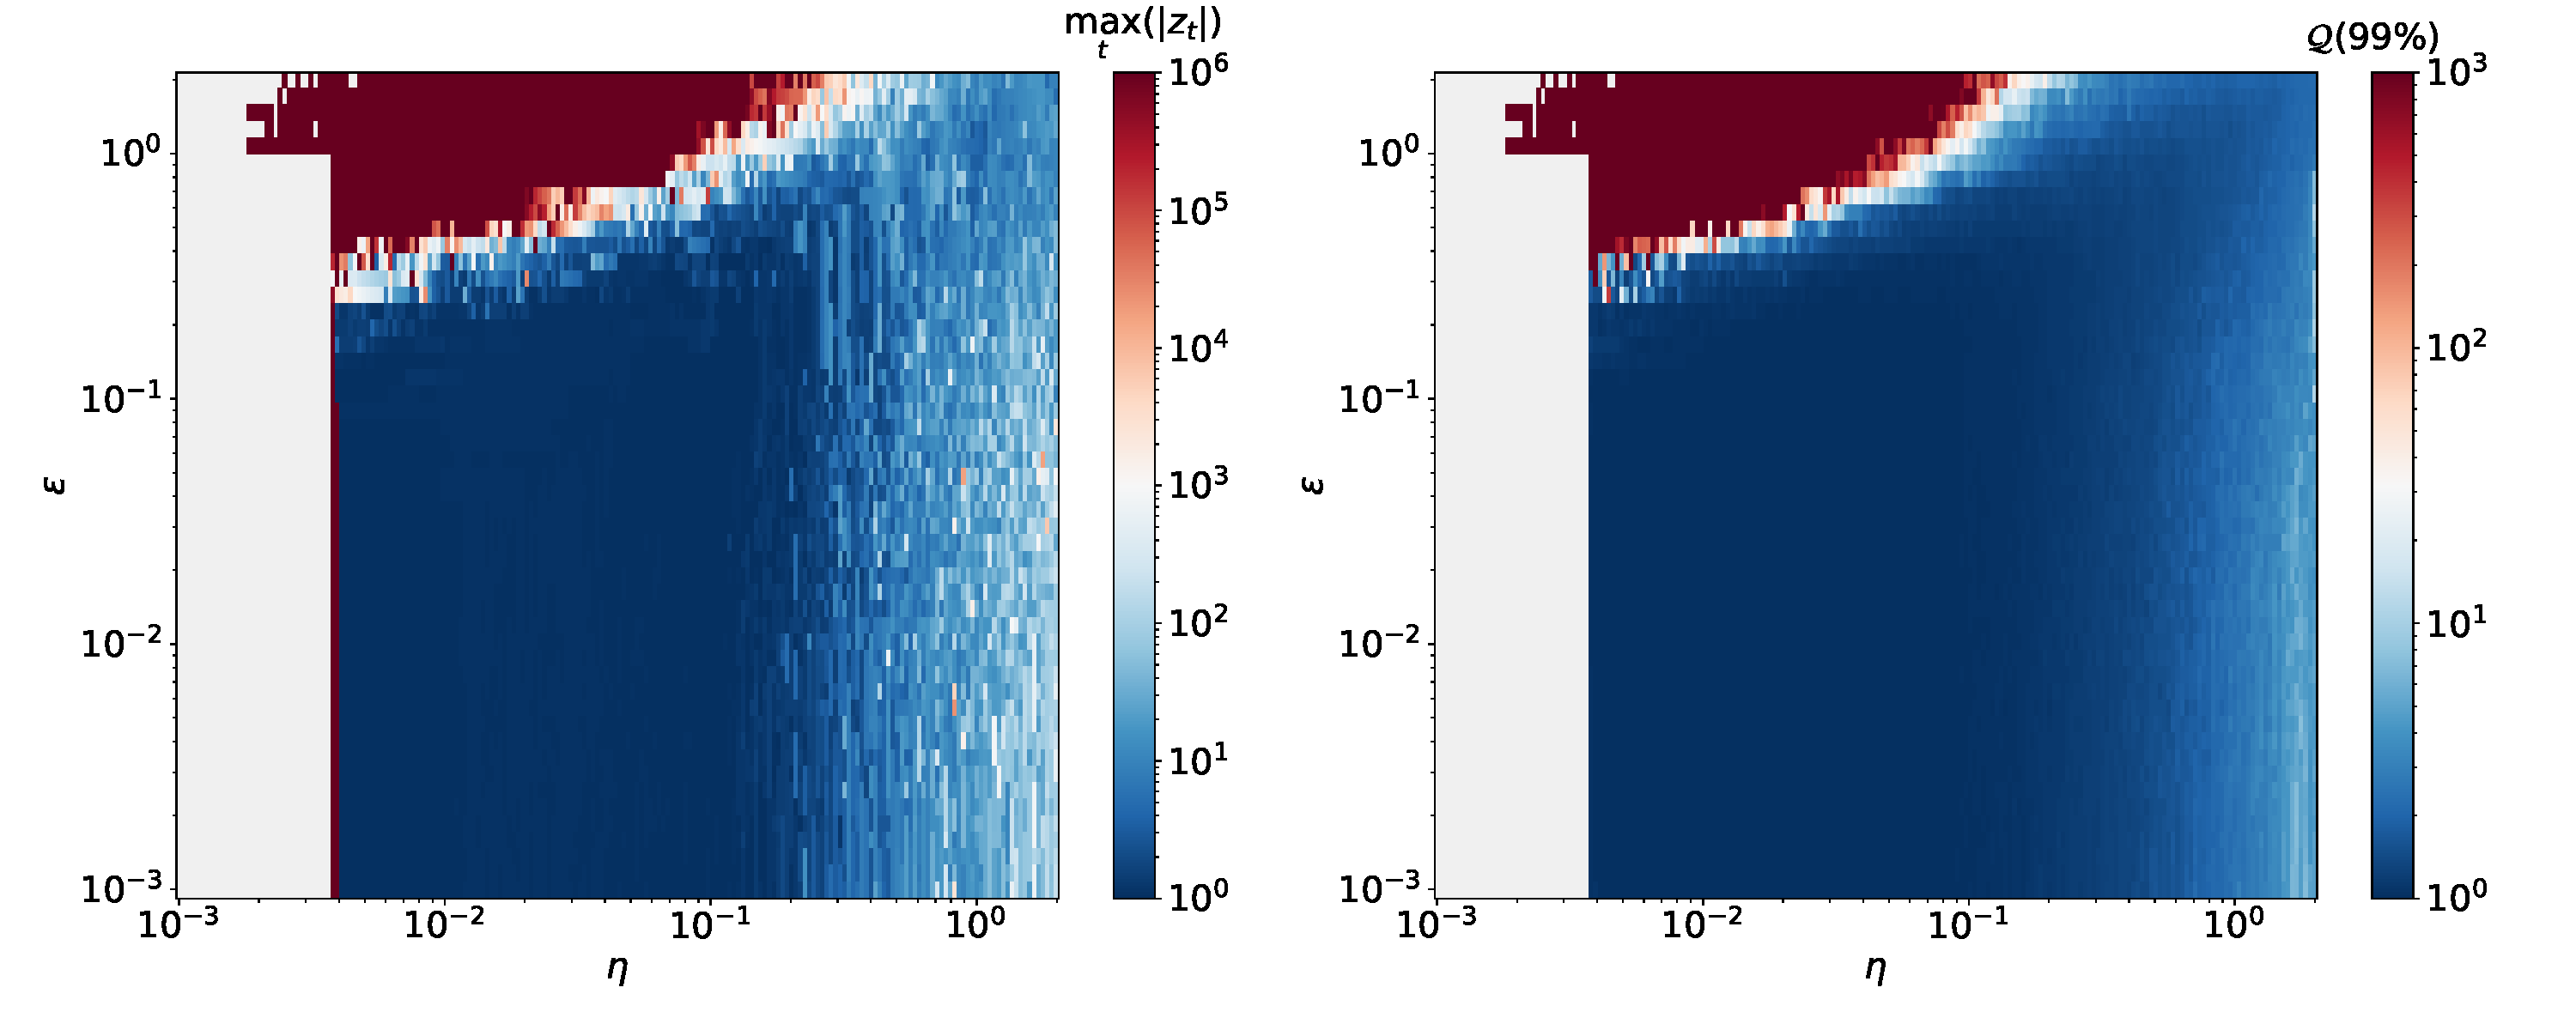
\includegraphics[width=1.2\textwidth]{Graphs/max_quant_eta-eps}}
	%\includegraphics[width=.5\textwidth]{example-image-a}
	\caption{Summary statistics of time series simulated with \eqref{eq:nc}: maximum value (Left) and $99\%-$quantile (Right) for logarithmically spaced $\eta$ and $\varepsilon$. Difference between them enlightens the magnitude of extreme (top $1\%$) deviations. Both quantities are normalized by their theoretical value for a normal distribution $\N(0,\sigma_0^2)$, $m_\N=3.84$ and $\Q_{\N}(99\%)=2.08$ (see \autoref{app:max_distrib}). $N=10^4$, $\alpha_0=2$, $\sigma_0^2=0.8$, $z_0=1$.}
	\label{fig:quant_max}	
\end{figure}


Both the maximum and last percentile exhibit an abrupt transition at $\eta^*=4\cdot10^{-3}$. They diverge below, and reach the theoretical value (see \autoref{app:max_distrib}) for a normal distribution\footnote{$m_\mathcal{N}=3.84$ for $N=10^4$ and $\mathcal{Q}_\mathcal{N}(99\%)=2.08$} $\mathcal{N}(0,\sigma_0^2)$ above. With smaller learning rate the estimator \eqref{eq:nc_eta} is updated by smaller steps and, therefore, takes more time to converge towards $\alpha_0$. With the initial condition $z_0=1$ and $\alpha_0=2$ the time series starts increasing, engaging \eqref{eq:nc_eta} from the beginning. As it stays above the origin, the dynamics reduces to $z_{t+1}=(\alpha_0-t\cdot\eta)z_t+\beta_t$. It becomes on average convergent ($\E{z_t/z_{t-1}}<1$) after $\sim(\alpha_0-1)/\eta$ time-steps (see Figure \ref{fig:nc_conv}).

\begin{figure}[h!]
\centering
	\centering
	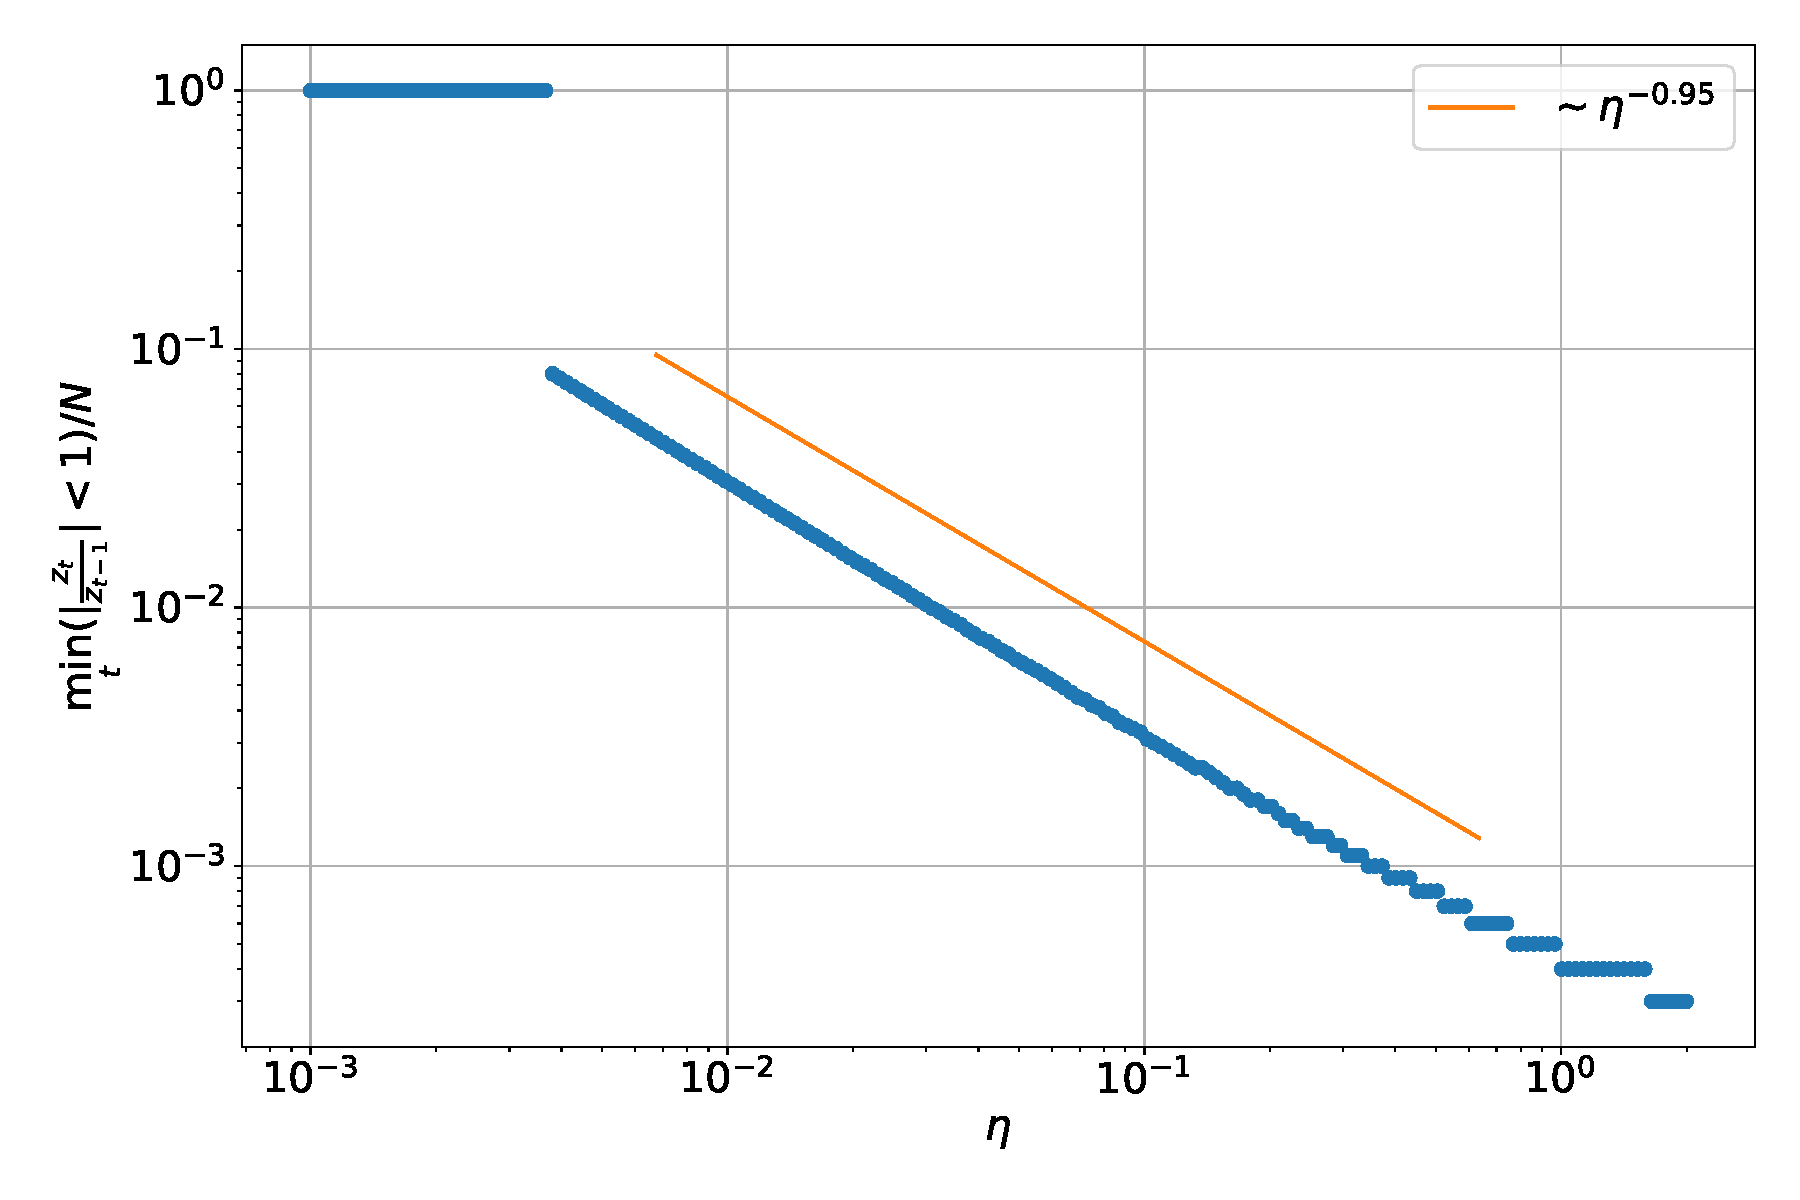
\includegraphics[width=.8\textwidth]{Graphs/nc_conv.pdf}
	\caption{Relative duration of the transient regime before the solution of \eqref{eq:nc} starts decreasing ($\min_t\{\abs{z_t/z_{t-1}}<1\}/N$), given $\eta$. In orange, reference line $\eta^{-0.95}$ fitting the predicted duration $(\alpha_0-1)/\eta$. The initial flat regime corresponds to diverging part: the dynamics is stuck on an explosive trajectory. $N=10^4$, $\alpha_0=2$, $\sigma_0^2=0.8$, $z_0=1$ and $\varepsilon=0.1$.}
	\label{fig:nc_conv}	
\end{figure}
 
 If $\eta$ is to small the excitation $(\alpha_0-c_t)$ therefore stays larger than one during many time-steps, putting the time series on an explosive track. Above $\eta^*$, the controller gets closer to $\alpha_0$ sufficiently early and prevents the time series from diverging, even though it may take a long time reach a stationary regime. For Figure \ref{fig:quant_max}, the first $1000$ time-steps ($10\%$ of total time) are omitted to focus on the stationary regime. This threshold obviously depends on $\alpha_0$, in a piecewise linear way  (Figure \ref{fig:eta_div_a0_s0}). Noise dependence exhibits a transition at $\sigma_0^2=1$. Above, noise is strong enough to compensate a large excitation factor $(\alpha_0-c_t)$, allowing $z_t$ to leave the initially divergent trajectory.

\begin{figure}[h!]
\centering
	\centering
	\makebox[\textwidth][c]{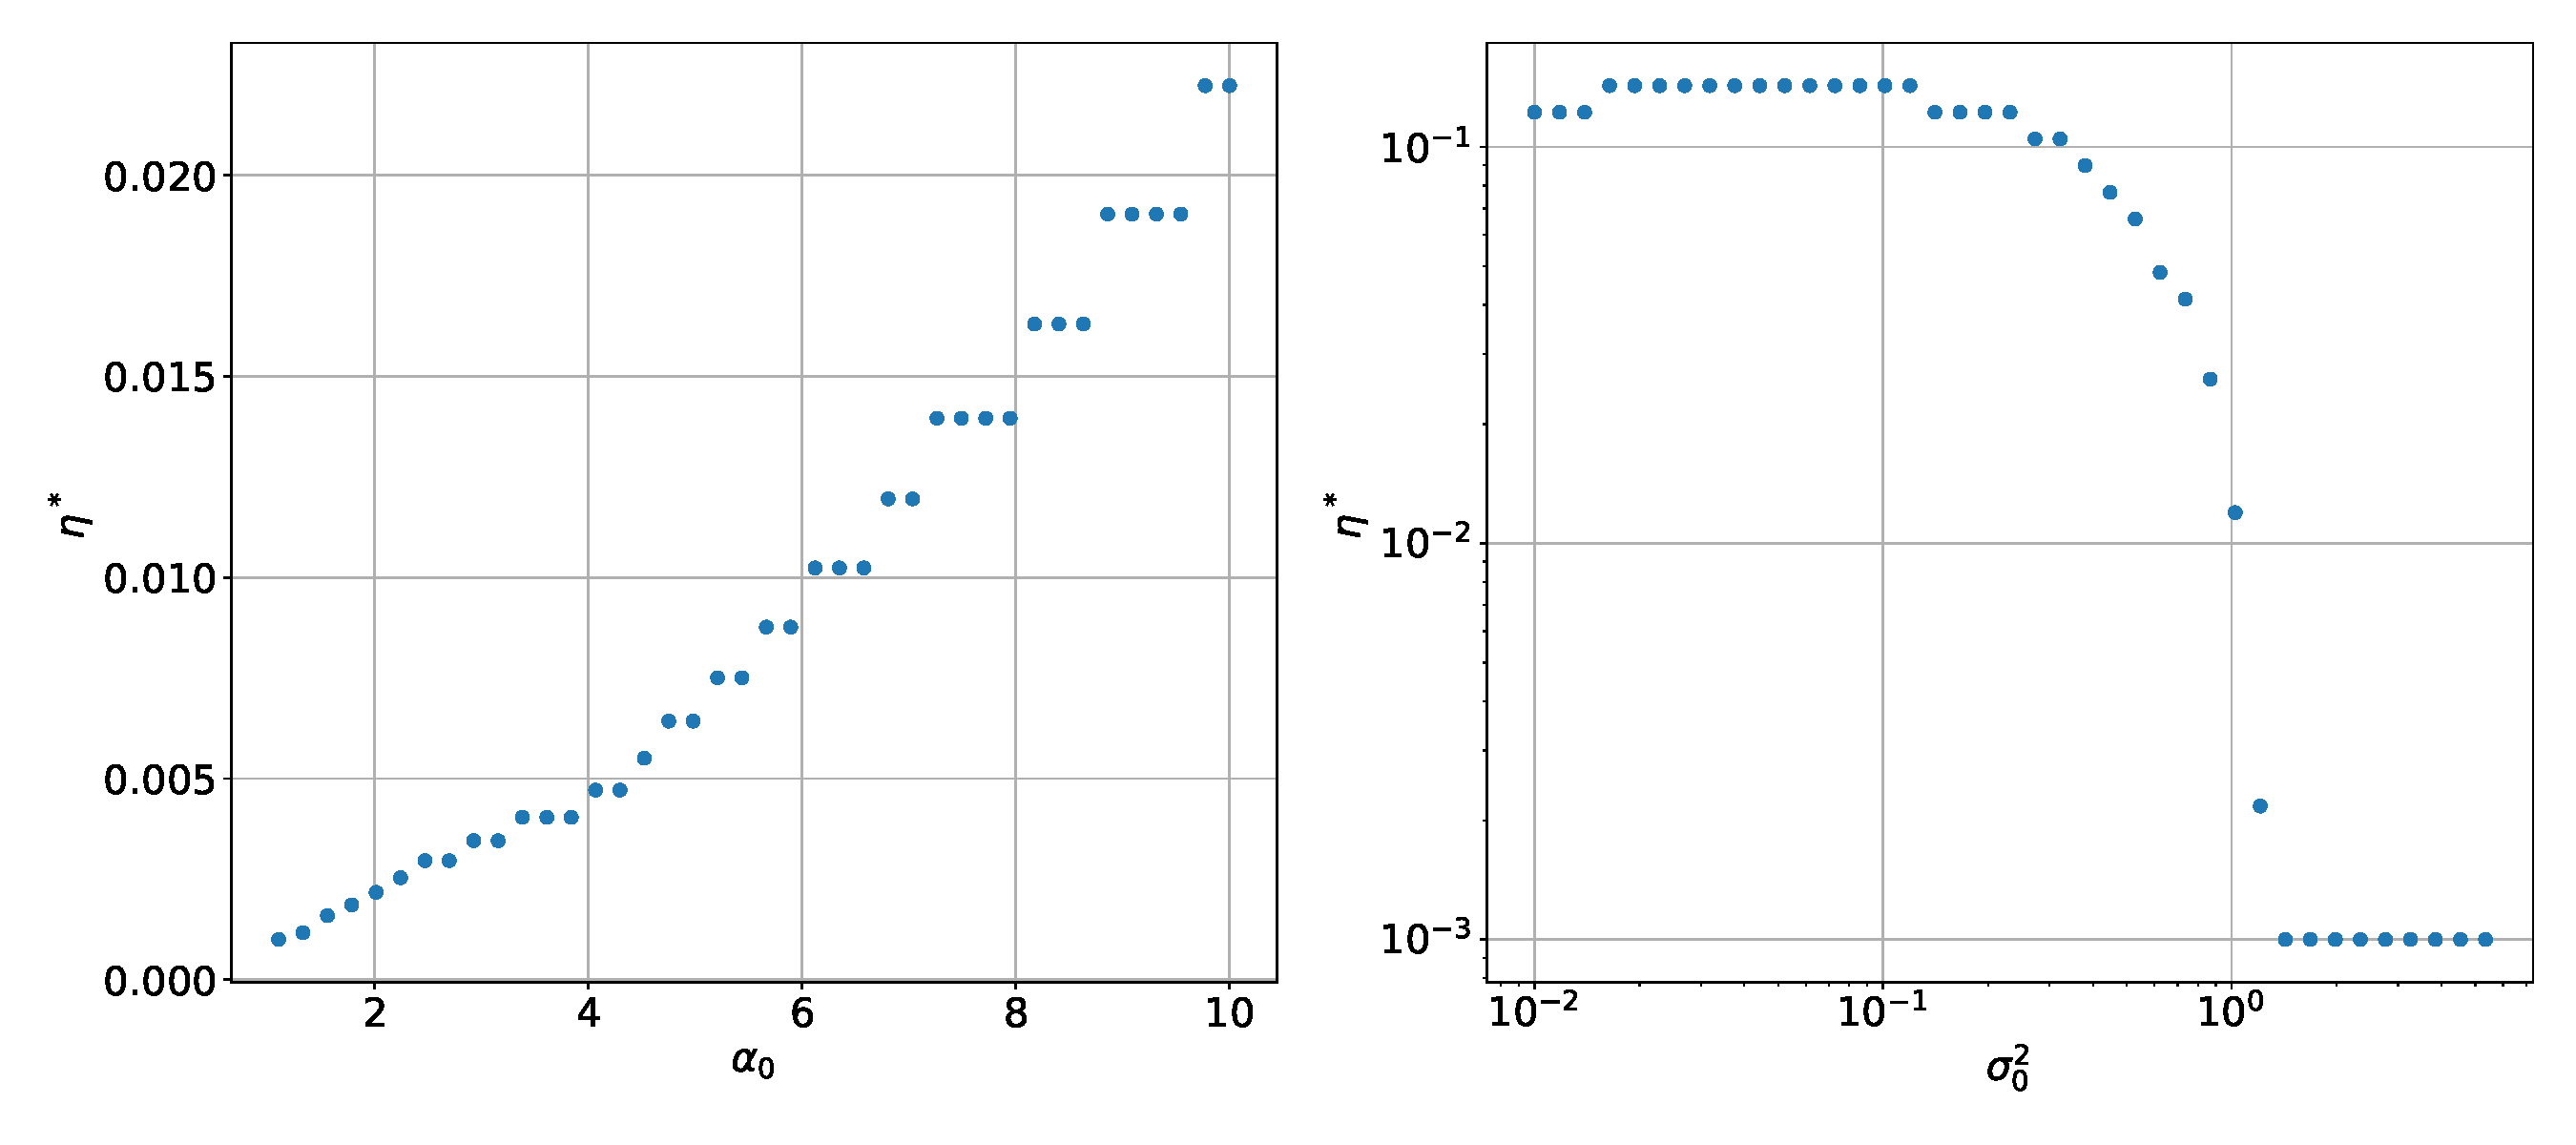
\includegraphics[width=1.1\textwidth]{Graphs/eta_div_a0_s0}}
	\caption{Threshold $\eta^*$ below which the dynamics always diverge, versus excitation parameter $\alpha_0$ (Left) and noise intensity $\sigma_0^2$ (Right). The linear relationship $\eta^*\sim\alpha_0$ comes from the estimator \eqref{eq:nc_eta}, but the transition around $\sigma_0^2=1$ is less trivial. After this threshold, noise is large enough to compensate the error due to a smaller learning rate. $N=10^4$, $\alpha_0=2$, $\sigma_0^2=0.8$, $z_0=1$ and $\varepsilon=0.1$.}%% TODO: rewrite last argument.
	\label{fig:eta_div_a0_s0}	
\end{figure}

Figure \ref{fig:quant_max_eps_fixed} shows again the maximum and $99\%-$quantile, for $\varepsilon=0.1$. A second transition becomes visible at $\eta\approx1.5\cdot10^{-1}$. Maximum value and last quantile both start increasing, but much slower for the latter. The increasing spread between them indicates that extreme deviations increase more rapidly than smaller ones.

\begin{figure}[h!]
\centering
	\centering
	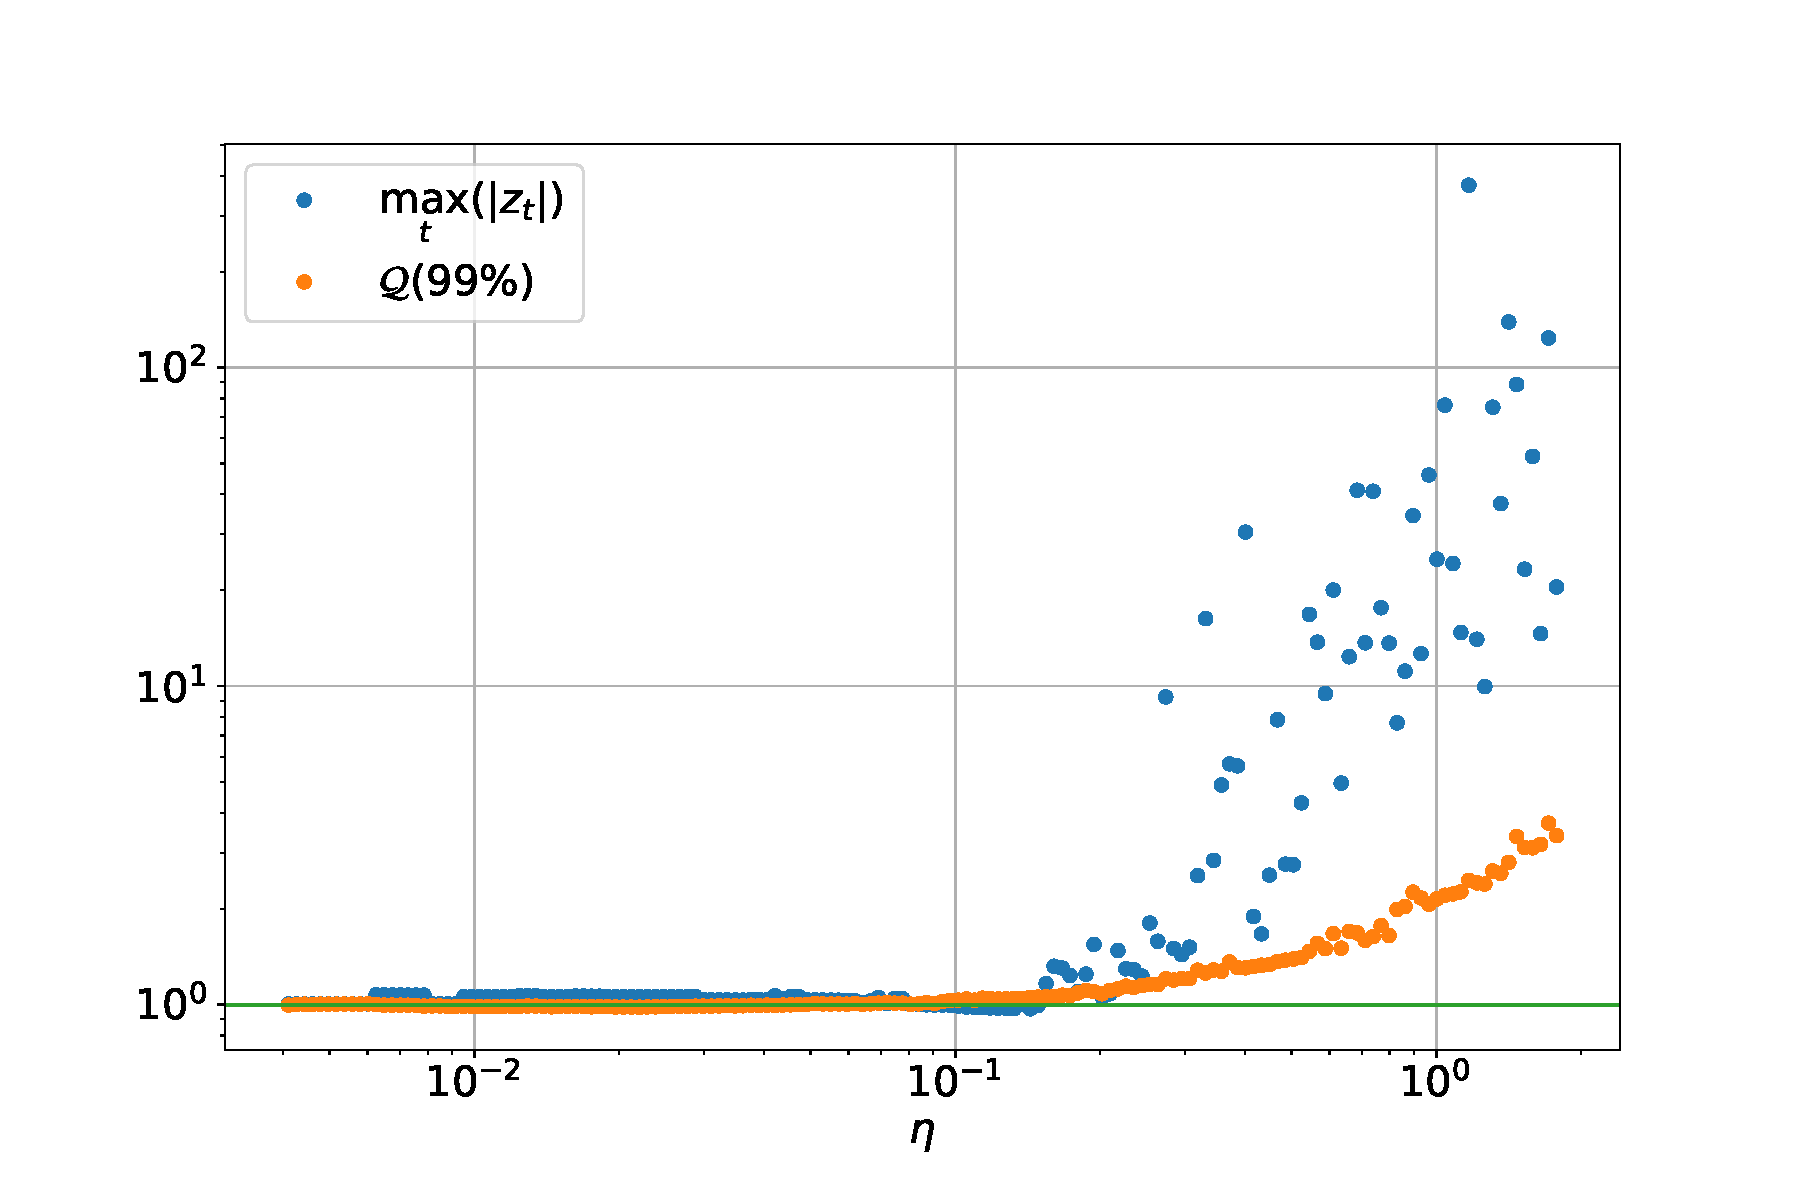
\includegraphics[width=.8\textwidth]{Graphs/quant_max_eps_fixed}
	\caption{Sectional view of Figure \ref{fig:quant_max} for $\varepsilon=0.1$ and $\eta>\eta^*=4\cdot10^{-3}$, showing the transition at $\eta=1.5\cdot10^{-1}$. The increasing spread between last percentile and maximum value indicates the appearance of a heavy tail.
	Both quantities are normalized by their theoretical value with a normal distribution for comparison ($m_\N=3.84$ and $\Q_{\N}(99\%)=2.08$, see \autoref{app:max_distrib}). $N=10^4$, $\alpha_0=2$, $\sigma_0^2=0.8$, $z_0=1$.}
	\label{fig:quant_max_eps_fixed}
\end{figure}


From those observations we have seen that several regime arise given $\varepsilon$ and $\eta$. In the "central" region $\varepsilon<1.5\cdot10^{-1}$ and $4\cdot10^{-3}<\eta\lesssim1.5\cdot10^{-1}$ both the maximum and last percentile of the time series are constant, close to their theoretical value for $\mathcal{N}(0,\sigma_0^2)$. For larger learning rate the tail of the distribution gets heavier; and the solution becomes totally divergent below $\eta^*$. Finally for $\varepsilon\gtrsim0.8$ distribution becomes closer to the power law obtained with original control \eqref{eq:map}. To confirm this observation Figure \ref{fig:mu_nc} shows the estimated tail exponent. The same behavior appear : in the "central" region the exponent is almost independent and close to $7$, indicating a rather thin tail\footnote{Exponent is estimated with Hill estimator, but the distribution in this region is closer to a Gaussian i.e. without a power tail.}. In the "outer" region ($\varepsilon\gtrsim0.8$ or $\eta\gtrsim 0.15$) it drops to $1$, as with the initial model.  


\begin{figure}[h!]
\centering
	\centering
	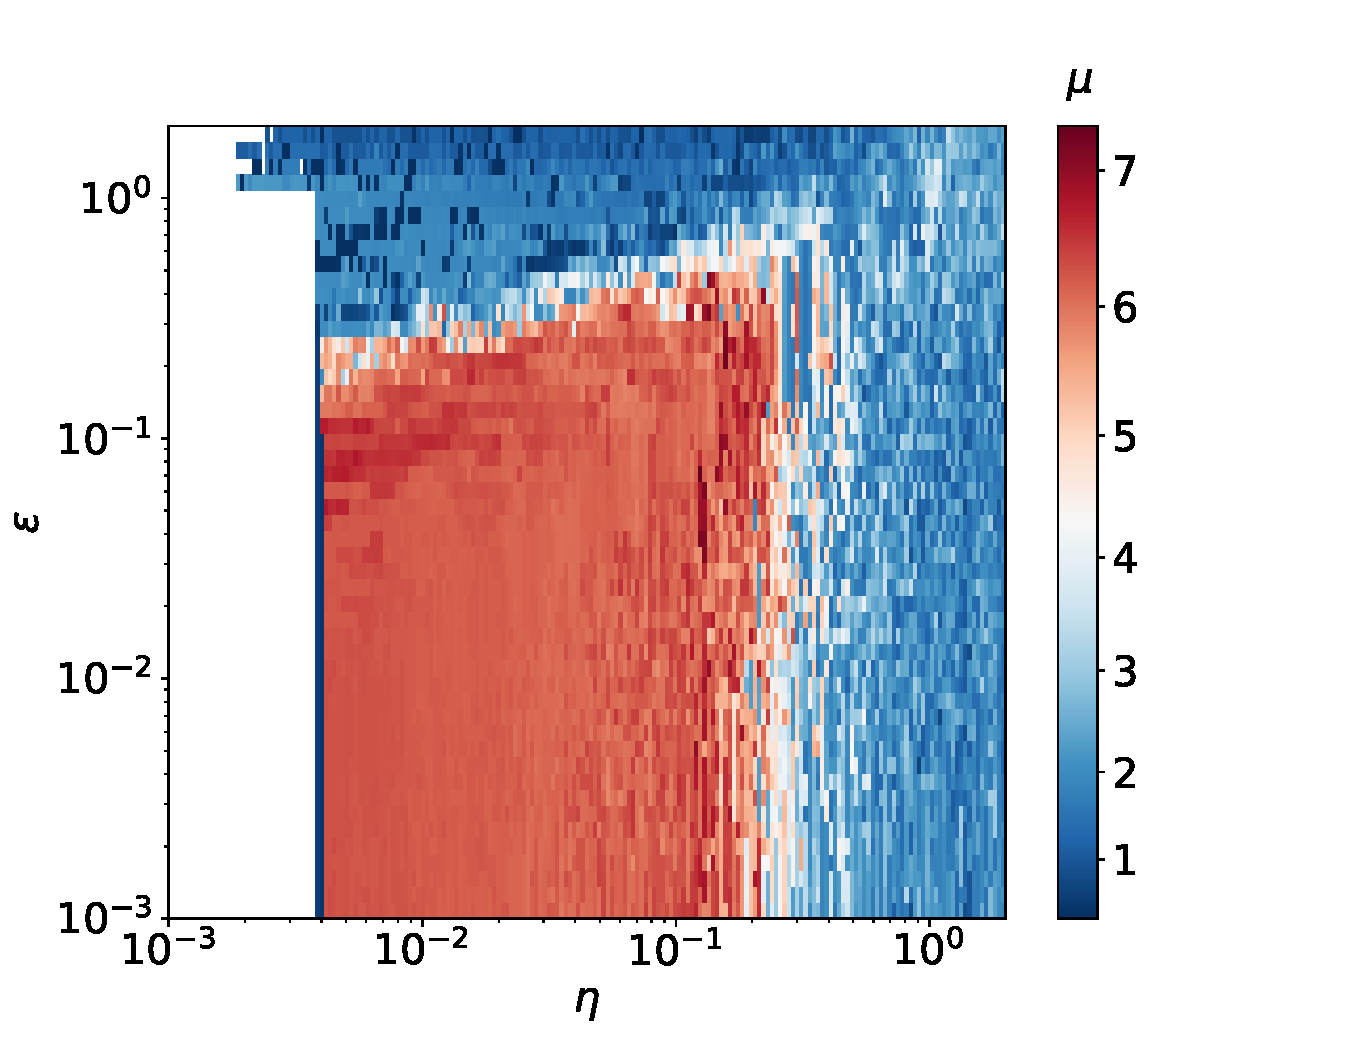
\includegraphics[width=1\textwidth]{Graphs/mu_nc}
	%\includegraphics[width=.5\textwidth]{example-image-a}
	\caption{Estimated exponent of the final distribution from \eqref{eq:nc}, using Hill estimator \cite{Hill75}. In the upper and right regions $P(z_t)$ is close to the power law obtained with original control \eqref{eq:tail_p(z)_n=1}, with exponent $\mu\approx1$. In the central region the distribution gets closer to a Gaussian therefore the exponent is much larger. $N=10^4$, $\alpha_0=2$, $\sigma_0^2=0.8$, $z_0=1$.}%%TODO: rewrite also
	\label{fig:mu_nc}	
\end{figure}

All those observations suggest to focus on the "central" region, where statistics is close to Gaussian distribution. For a deeper analysis of the final distribution we select $\varepsilon=0.1$ and $\eta=0.05$. Figure \ref{fig:ts_n1_nc} compares the solution of the original MLE control with the proposed control. Figure \ref{fig:dist_n1_nc} shows $P_>(z_t)$ in both case. The distribution with modified control is indeed Gaussian. Kolmogorov-Smirnov test gives a distance $1.17\cdot10^{-3}$ with $p-$value $0.49$, meaning that the solution is very likely normally distributed.


The modification proposed achieves optimal control, yielding a Gaussian distribution without large deviations ($\max{z_t}=4.8$).

\begin{figure}[h!]
\centering
	\centering
	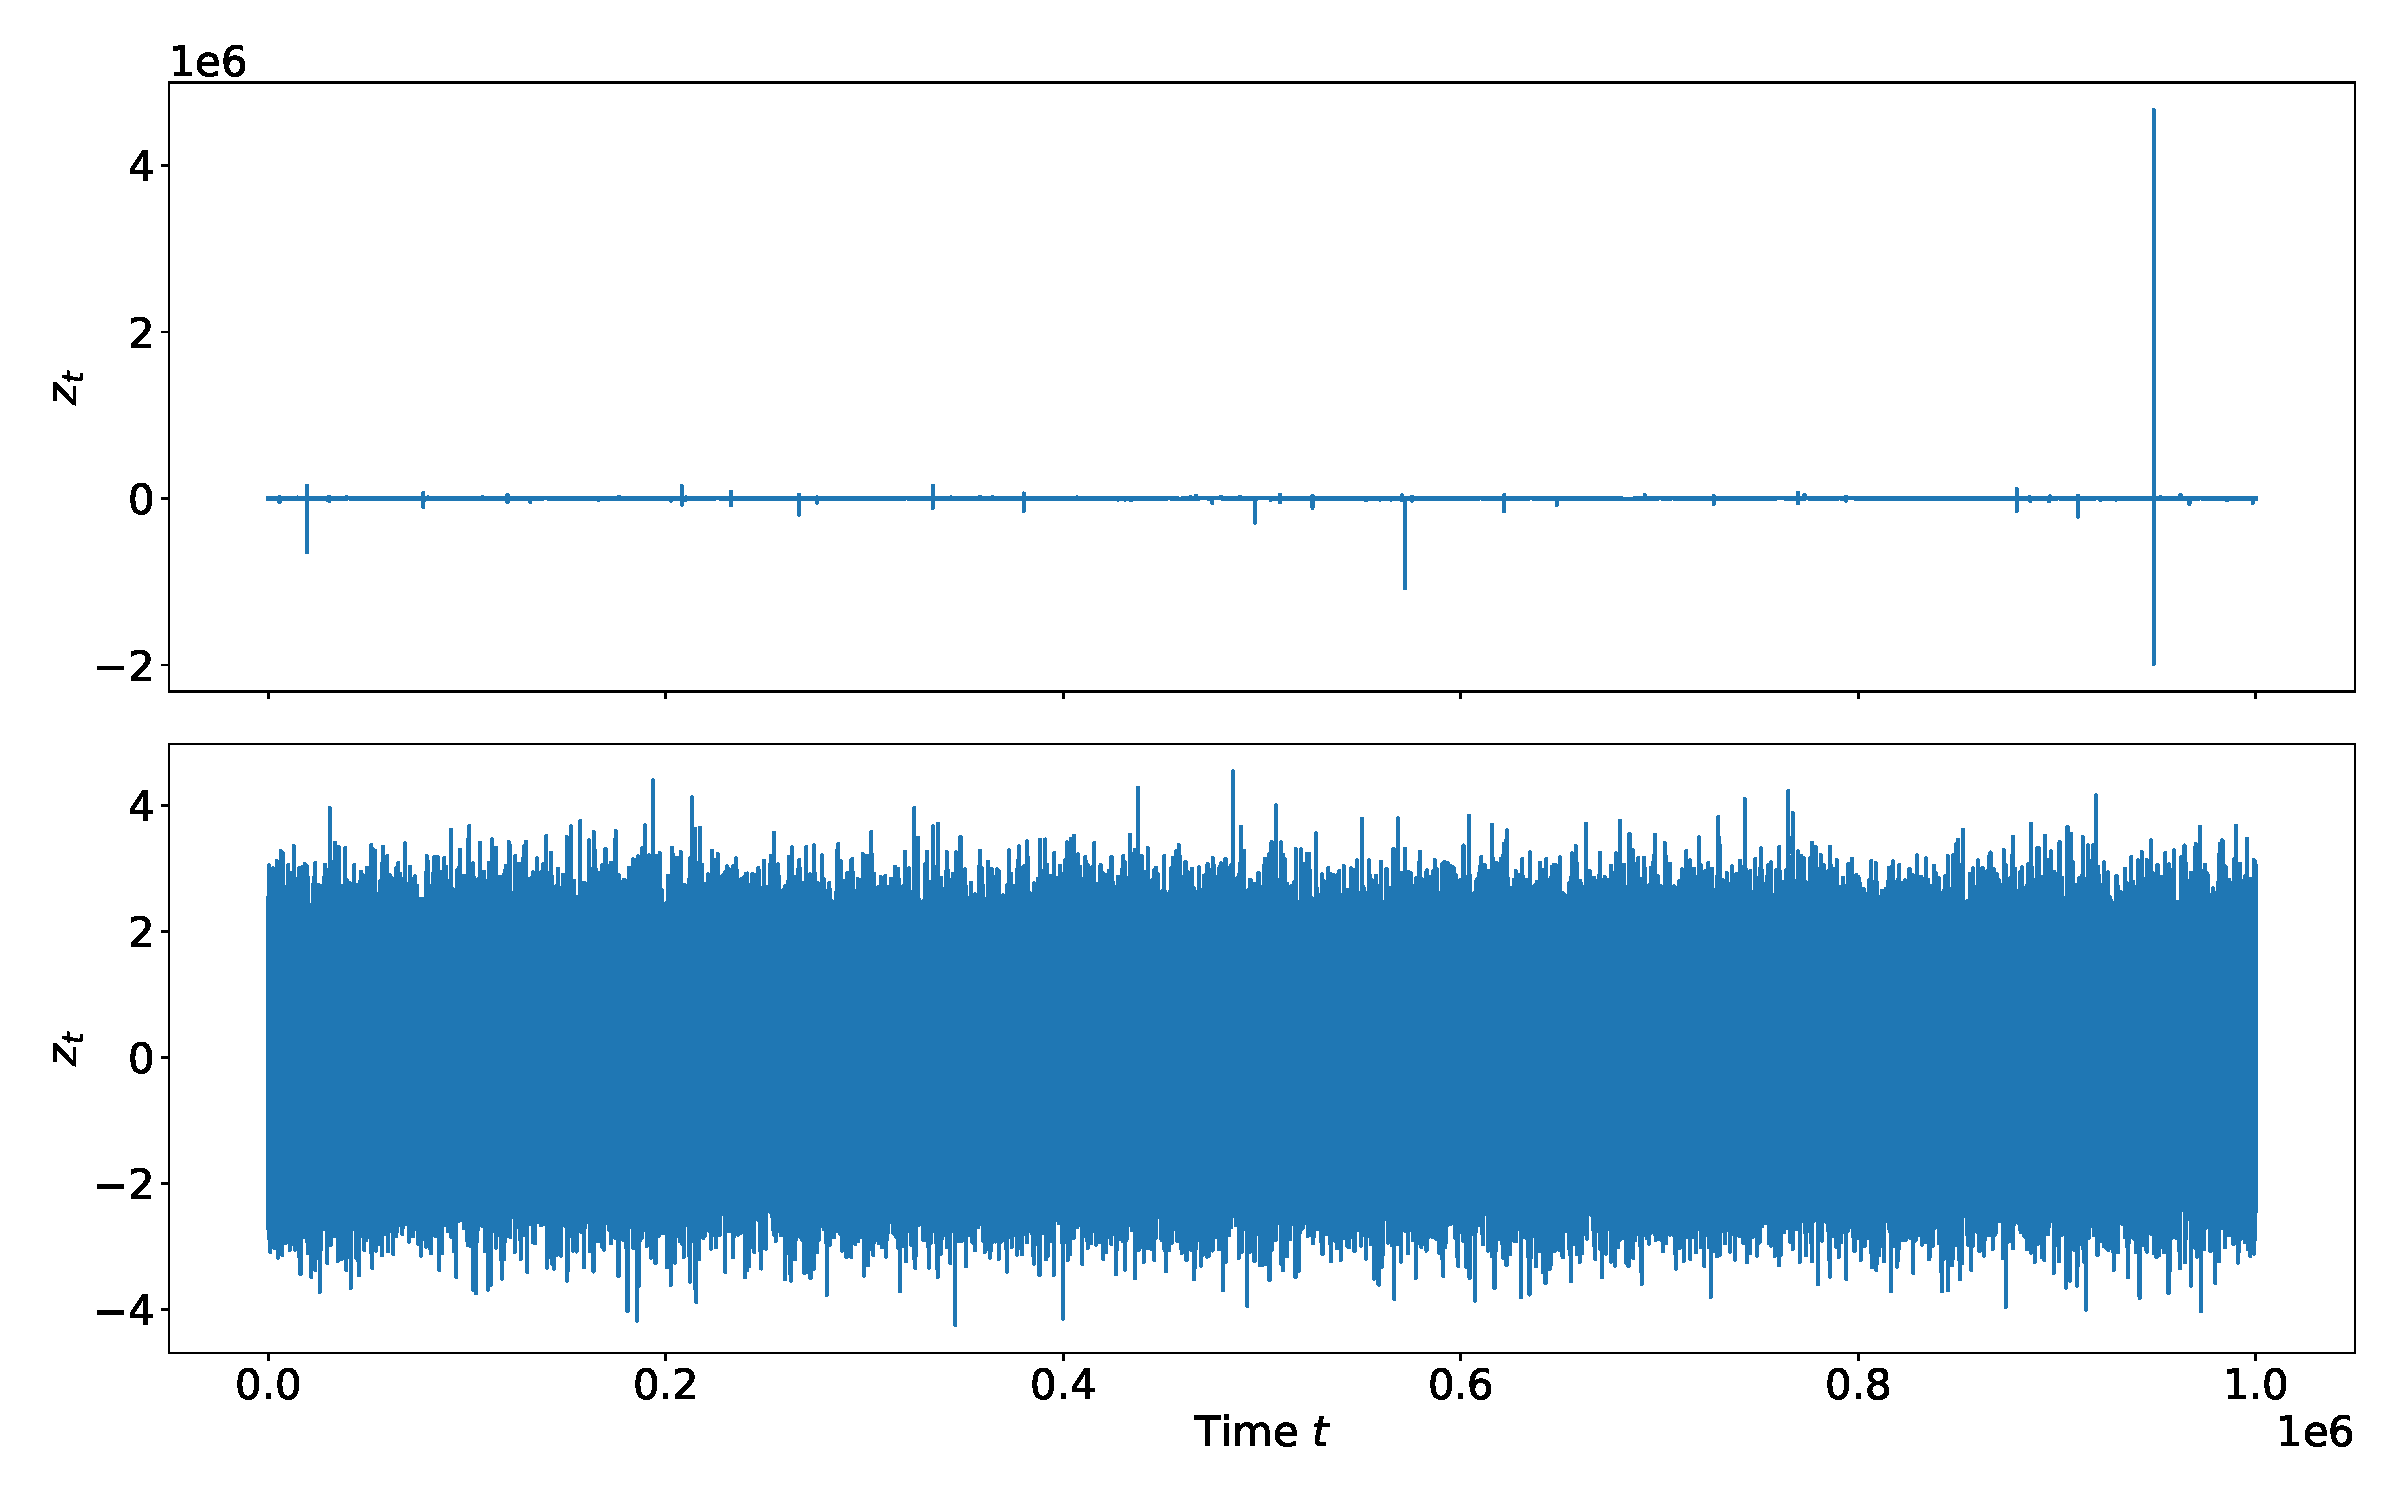
\includegraphics[width=1\textwidth]{Graphs/ts_n1_nc}
	%\includegraphics[width=.5\textwidth]{example-image-a}
	\caption{Numerical simulations of \eqref{eq:map} with the original MLE controller \eqref{eq:controller_mle_n} (Upper) and proposed modification \eqref{eq:nc} (Lower), for $\varepsilon=0.1$ and $\eta=0.05$. Added regularization achieves to prevent large deviations. All parameters are identical: $\alpha_0=2$, $\sigma_0^2=0.8$, $z_0=1$, $N=10^6$.}
	\label{fig:ts_n1_nc}	
\end{figure}


\begin{figure}[h!]%% TODO : eta as free parameter ?
\centering
	\centering
	\makebox[\textwidth][c]{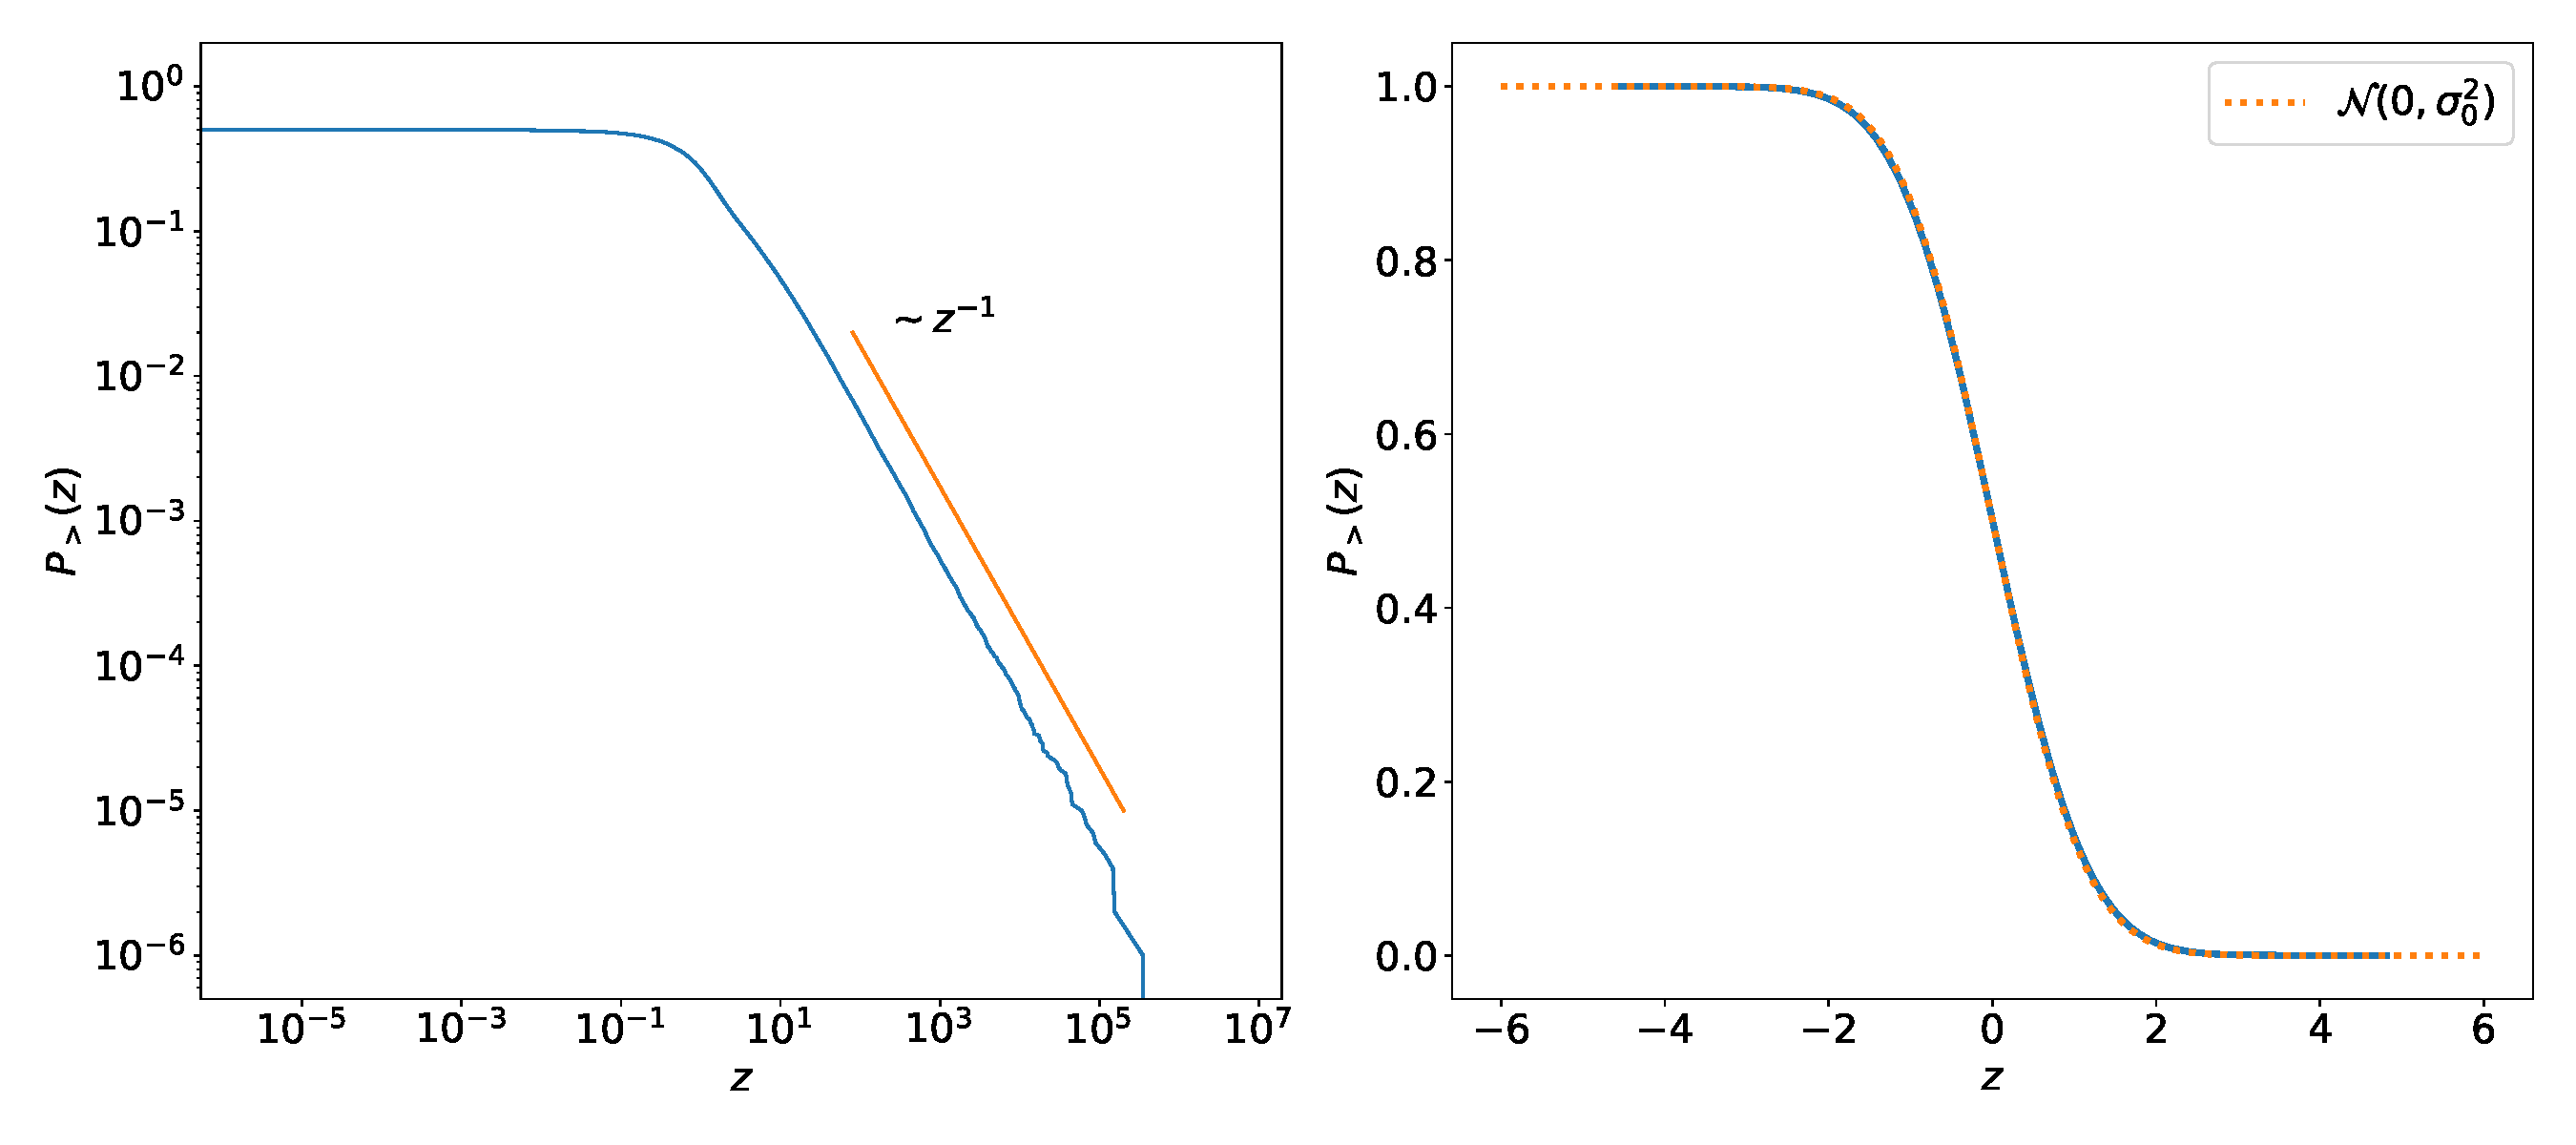
\includegraphics[width=1.1\textwidth]{Graphs/dist_n1_nc}}
	%\includegraphics[width=.5\textwidth]{example-image-a}
	\caption{CCDF of simulations from Figure \ref{fig:ts_n1_nc}. Original MLE controller (Left) and proposed modification (Right), with $\varepsilon=0.1$ and $\eta=0.05$. Final distribution with regularization is very close to $\N(0,\sigma_0^2)$ (orange), indicating optimal control. 
	All parameters are identical: $\alpha_0=2$, $\sigma_0^2=0.8$, $z_0=1$, $N=10^6$. Left plot is in log-log to make the power law visible.}
	\label{fig:dist_n1_nc}	
\end{figure}

\section{Simplification of the model}
All those observations confirm that the modification proposed is indeed able to make the controller optimal, in the sense that $z_t\sim =\mathcal{N}(0,\sigma_0^2)$. However this result depends heavily on the choice of $\varepsilon$ and $\eta$. Even though we obtained good result with $(\varepsilon,\eta)=(0.1,0.5)$, this choice is arbitrary. By reducing to one the number of free parameters, it is easier to numerically optimize the value.

A first simplification could be to set $\eta=\varepsilon$, as results are typically better along this line for large $\varepsilon$ (data not shown). The map then reduces to
\begin{equation}\label{eq:simp-1}
		z_{t+1}=\left[\alpha_0-c_{t-1}-\sign{\frac{z_t}{z_{t-1}}}\min\left(\eta,\abs{\frac{z_t}{z_{t-1}}}\right)\right] z_t + \beta_t.
\end{equation}
Similarly, simulations have shown that below some value the distribution is independent of $\varepsilon$. Another simplification could thus be to forget totally the original controller, by setting $\varepsilon=0$
\begin{equation}\label{eq:simp-2}
		z_{t+1}=\left[\alpha_0-c_{t-1}-\eta\,\sign{\frac{z_t}{z_{t-1}}}\right] z_t + \beta_t.
\end{equation}
This control is still adaptive as it keeps track of the descent direction $\sign{z_t/z_{t-1}}$, but always moves by constant steps $\eta$. In both case, having a unique parameter makes the model simpler. It is numerically possible to evaluate $\eta^*$, that minimize Kolmogorov-Smirnov distance $D_{KS}$ with $\mathcal{N}(0,\sigma_0^2)$ (Figure \ref{fig:special_cases}). The first model ($\eta=\varepsilon$) gives an acceptable $p-$value for a wider range of $\eta$, but both achieve optimal control.
\begin{figure}[h!]
\centering	
\makebox[\textwidth][c]{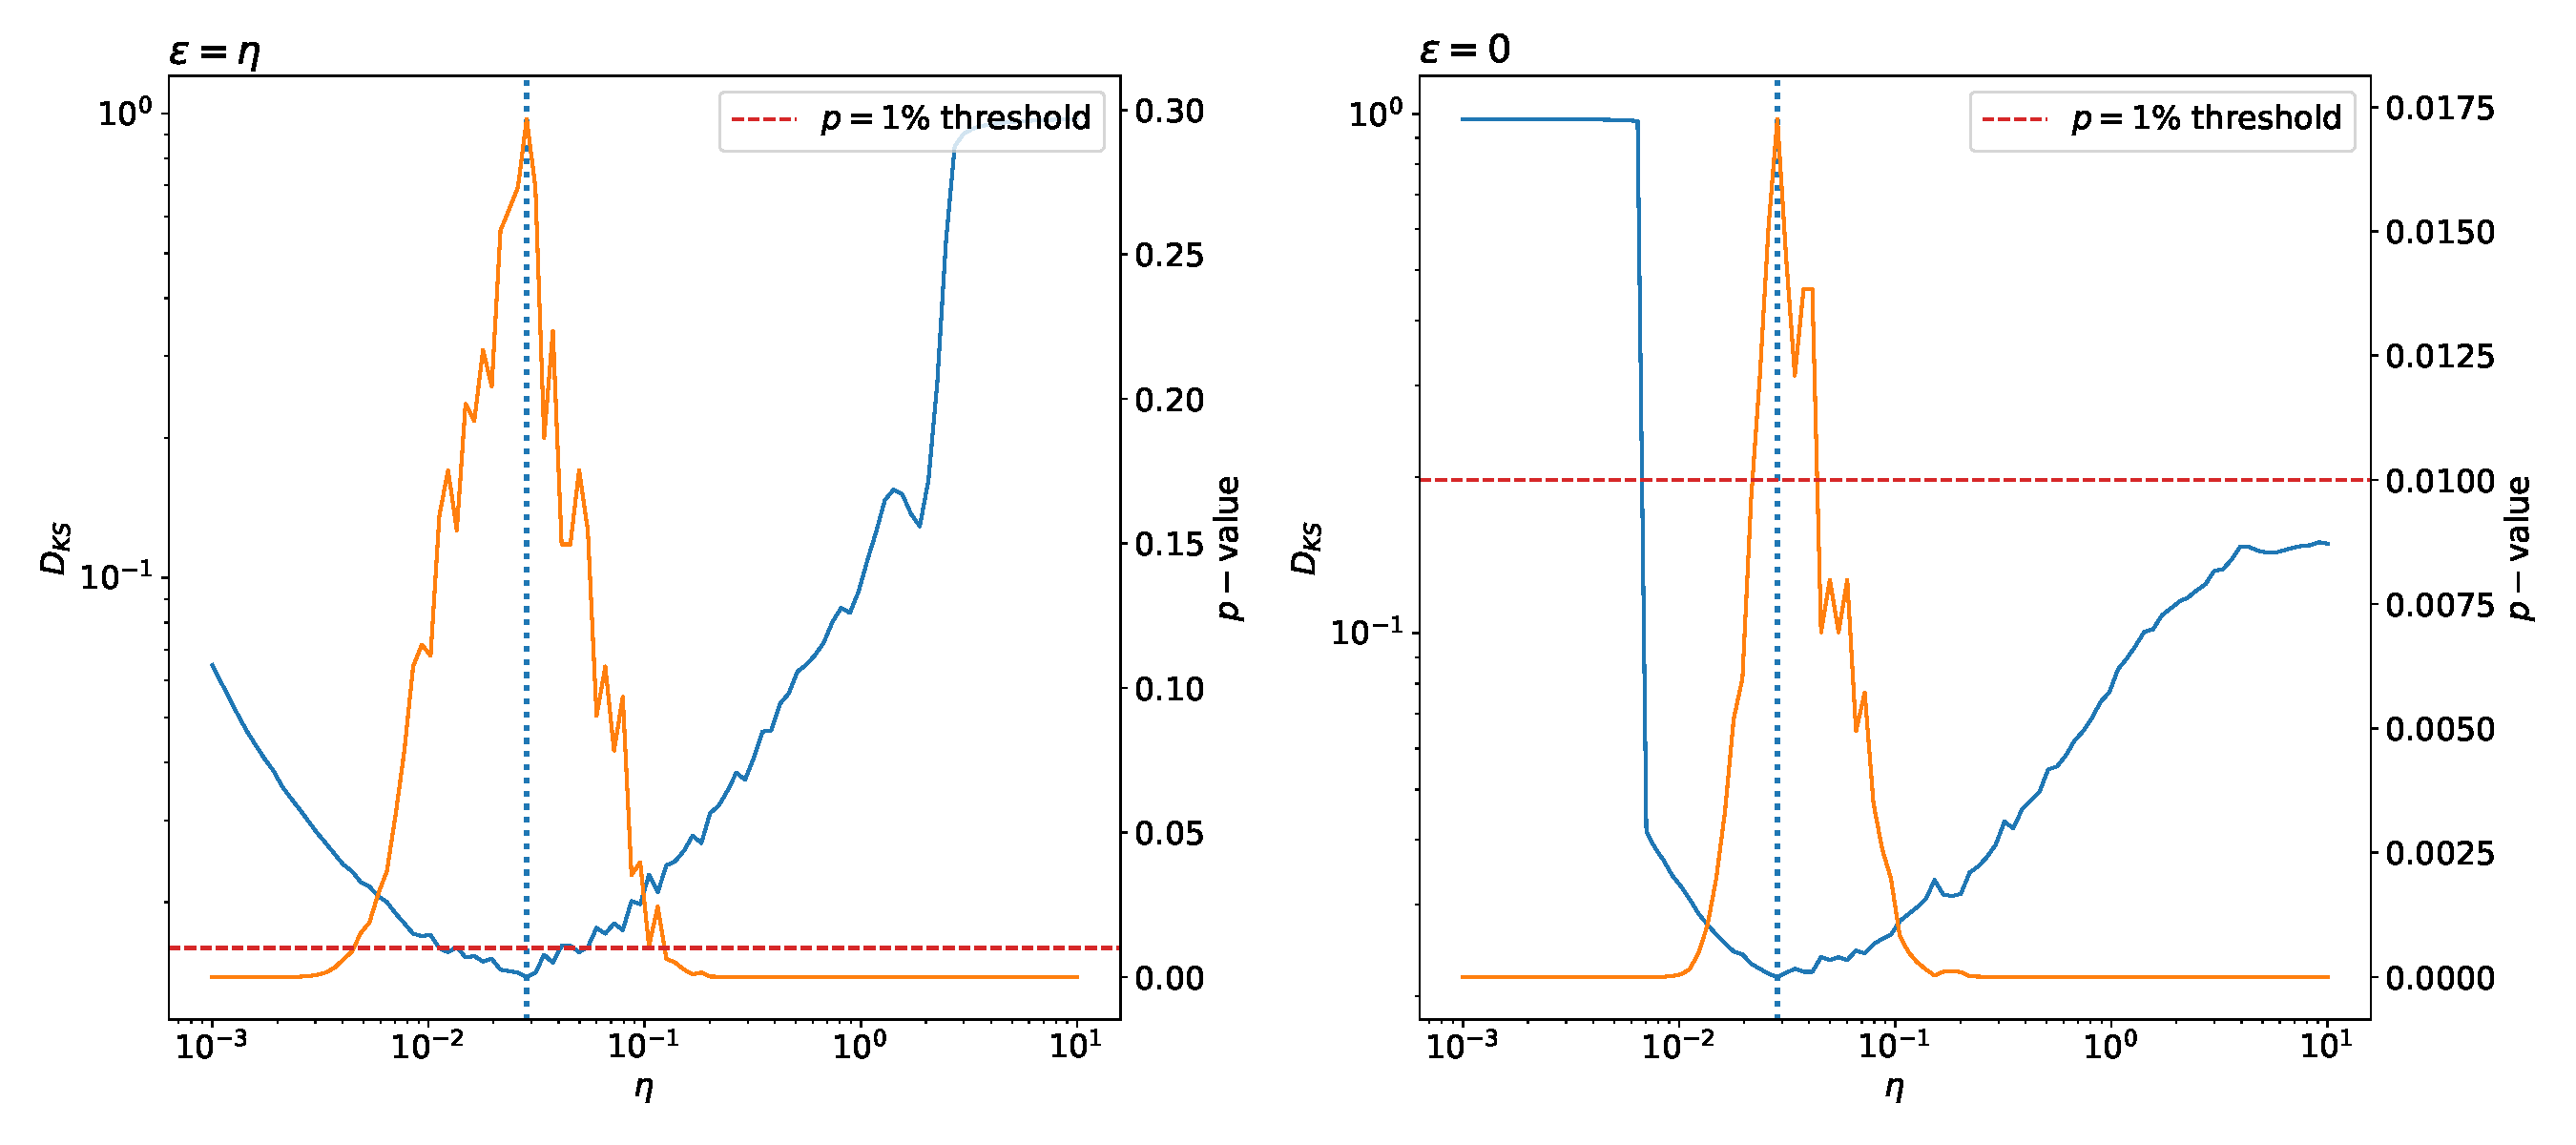
\includegraphics[width=1.1\textwidth]{Graphs/special_cases.pdf}}
\caption{KS distance (left axis, blue) and $p-$value (right axis, orange) for the two simplifications proposed (\ref{eq:simp-1},~\ref{eq:simp-2}). Red dashed line indicates the threshold $p=1\%$, above which the hypothesis that $P(z_t)$ is normally distributed is acceptable. Distance between the two distributions are similar in both case, but the first proposition $\varepsilon=\eta$ is normally distributed for a broader range of $\eta$, with better $p-$value. The optimal learning rates are respectively $\eta_{opt}=1.35\cdot10^{-2}$ and $\eta_{opt}=1.96\cdot10^{-2}$.
$N=10^4$, $\alpha_0=2$, $\sigma_0^2=0.8$, $z_0=1$.}
\label{fig:special_cases}	
\end{figure}


Distribution $P(z_t)$ is not a power law anymore, thus it has finite variance. In the case $\varepsilon=0$ it reads
\begin{align}
	\expval{z_{t+1}^2}&=\expval{\left[\left(\alpha_0-c_{t-1}-\eta\,\sign{\frac{z_t}{z_{t-1}}}\right)z_t +\beta_t\right]^2}.
\end{align}
Thanks to the properties of noise we expand it as
\begin{align}
	\expval{z_{t+1}^2}&=\expval{\left(\alpha_0-c_{t-1}-\eta\,\sign{\frac{z_t}{z_{t-1}}}\right)^2z_t^2}+\sigma_0^2\\
	&=\expval{\left(\alpha_0-c_{t-1}\right)^2z_t^2}+\eta^2\expval{z_t^2}-2\eta\expval{z_t^2\sign{\frac{z_t}{z_{t-1}}}(\alpha_0-c_{t-1})}+\sigma_0^2.
\end{align}
\begin{comment}
\end{comment}
The minimal value is reached for 
\begin{equation}
	0=\left.\pdv{\expval{z_{t+1}^2}}{\eta}\right\vert_{\eta_{opt}}=2\eta_{opt}\expval{z_t^2}-2\expval{z_t^2\,\sign{\frac{z_t}{z_{t-1}}}(\alpha_0-c_{t-1})},
\end{equation}
i.e.
\begin{equation}
	\eta_{opt}=	\sigma_0^2\frac{\expval{z_t^2\,\sign{\frac{z_t}{z_{t-1}}}(\alpha_0-c_{t-1})}}{\expval{z_t^2}}.
\end{equation}
This value cannot be computed ex ante as it depends on hidden parameters. If available, one could use a "train" set to optimize the parameters first.




\end{document}